
\chapter{ಪುನರಾಗಮನ –ಎವರೆಸ್ಟ್​ರ ದಶಕ ಆರಂಭ}

ನಂತರ \enginline{1830}ರಲ್ಲಿ ಭಾರತಕ್ಕೆ ಮರಳಿದರು. ಈ ಸಮಯದಲ್ಲಿ ಎವರೆಸ್ಟ್​ರವರು ಸರ್ವೆ ಆಫ್​ ಇಂಡಿಯಾ ಮಹಾ ಸಂಸ್ಥೆಯನ್ನು ಇನ್ನೂ ಸಮರ್ಥವಾಗಿ ಕಟ್ಟಲು ನಿರ್ಧರಿಸಿ, ಅದರ ಹಿಂದಿನ ವ್ಯವಸ್ಥೆಯನ್ನು ಬದಲಾವಣೆ ಮಾಡಿದರು. ಹಳೆಯ ವಿಧಾನಗಳಿಗೆ ಅಮೂಲ್ಯ ಬದಲಾವಣೆ ತಂದರು. ಈ ಅವಧಿಯಲ್ಲಿ ಅವರು ಮುಖ್ಯವಾಗಿ ಗ್ರೇಟ್​ ಟ್ರಿಗನಮಿಟ್ರಿಕಲ್​ ಸರ್ವೇ ಆಫ್​ ಇಂಡಿಯಾದ ಪುನರ್​ರಚನೆಗೆ ಗಮನ ಕೊಟ್ಟರು.

ಸರ್ವೇಯ ಯಶಸ್ಸು ಮತ್ತು ಶ್ರೇಷ್ಠತೆ ಇರುವುದು ಉಪಕರಣ ತಯಾರಕರು ಸಾಧಿಸಿದ ನಿಖರತೆ ಮೇಲೆ. ನಿಖರವಾದ ಸರ್ವೇಗೆ ಉಪಕರಣಗಳ ಗುಣಮಟ್ಟವೂ ಸಹ ಬಹು ಮುಖ್ಯವಾಗುತ್ತದೆ. ಕೆಲವೊಮ್ಮೆ, ಸರ್ವೇ ಉಪಕರಣಗಳು ಅವುಗಳ ಡಿಸೈನ್​ನಲ್ಲಾಗಲೀ, ಕಾರ್ಯ ಕೌಶಲ್ಯದಲ್ಲಾಗಲೀ, ಕಾರ್ಯ ತತ್ವದಲ್ಲಾಗಲೀ, ರಚಿಸಿದ ಲೋಹ ವಸ್ತುವಿನಲ್ಲಾಗಲೀ ಹಾಗು ಹೆಚ್ಚಿನ ಸಂದರ್ಭಗಳಲ್ಲಿ ಈ ಎಲ್ಲಾ ಮಿಶ್ರಿತ ವಿಷಯಗಳಲ್ಲಿಯೂ ದೋಷಯುತವಾಗಿರುತ್ತವೆ. ಪ್ಯಾರಲಲ್​ ರೂಲರಿನಿಂದ ಎಳೆದ ಗೆರೆಗಳು ಪಾರಲಲ್​ ಆಗಿರಬೇಕು. ಆದರೆ ಅವುಗಳು ಪ್ಯಾರಲಲ್​ ಆಗಿರುವುದಿಲ್ಲ. ಪ್ರೊಟ್ರಾಕ್ಟರ್​, ಸ್ಕೇಲು, ಲೆವಲಿಂಗ್​ ಸ್ಟಾಫ್​ಗಳು ಇವುಗಳಲ್ಲಿರುವ ಗೆರೆಗಳು ನಿಖರವಾಗಿ ಗ್ರಾಜ್ಯುಯೇಷನ್​ ಆಗಿರಬೇಕು. ಆದರೆ ಅವುಗಳೂ ತಪ್ಪಾಗಿ ಗ್ರಾಜ್ಯುಯೇಷನ್​ ಆಗಿರುತ್ತವೆ. ಬಾರೋಮೀಟರ್​, ಥಿಯಡೋಲೈಟ್​ಗಳು ದೋಷಮಯ ಆಗಿರುತ್ತವೆ. ಕೆಲವೊಮ್ಮೆ ನಿರಂತರ ಬಳಕೆಯಿಂದಲೂ ಸಹ ಉಪಕರಣಗಳು ದೋಷಯುತ ಆಗಿರುತ್ತವೆ. ಆದ್ದರಿಂದ ಸರ್ವೇ ಉಪಕರಣಗಳಲ್ಲಿನ ಈ ಎಲ್ಲಾ ಮುಖ್ಯ ದೋಷಗಳನ್ನು ಸುಧಾರಿಸಬೇಕು, ಸರಿಪಡಿಸಬೇಕು. ಉಪಕರಣದಲ್ಲಿ ಅಂತಿಮ ಎಂಬುದಿಲ್ಲ. ಸಿದ್ಧ ಮಾದರಿ, ರಿಪೇರಿಯೇ ಬೇಡ ಎನ್ನುವಂತಹ ಉಪಕರಣ ತಯಾರಿಕೆಯು ಸರ್ವೇ ಕ್ಷೇತ್ರದಲ್ಲಿ ಇಲ್ಲ. ವಿಜ್ಞಾನದಲ್ಲಿ ಹೊಸ ಹೊಸ ಶೋಧ ಆದಂತೆಲ್ಲಾ, ಹೊಸ ತಂತ್ರಜ್ಞಾನ ಬೆಳೆದಂತೆಲ್ಲಾ, ಉಪಕರಣಗಳು ತಮ್ಮ ರೂಪ ಮತ್ತು ಕಾರ್ಯತತ್ವದಲ್ಲಿ ಸದಾ ಬದಲಾಗುತ್ತಾ, ಹೊಸ ವಿನ್ಯಾಸಅ ತಾಳುತ್ತಾ ಇರುತ್ತವೆ. ಬದಲಾದ ಸಮಯ ಸನ್ನಿವೇಶ ತಂತ್ರಜ್ಞಾನಗಳಿಗೆ ಅನುಗುಣವಾಗಿ ಸರ್ವೇಯ ಉಪಕರಣದಲ್ಲೂ ಸುಧಾರಣೆೆಯನ್ನು ಅನಿವಾರ್ಯವಾಗಿ ಮಾಡಿಕೊಳ್ಳಬೇಕಾಗುತ್ತದೆ.

ಈ ಕಾರಣಕ್ಕೆ ಪ್ರಮುಖ ಅಂಶವಾದ ನಿಖರ ಸರ್ವೇ ಉಪಕರಣಗಳ ತಯಾರಿಕೆ ಮತ್ತು ಅವುಗಳ ನಿರ್ವಹಣೆಯ ಬಗ್ಗೆ ಎವರೆಸ್ಟ್​ರವರು ಒತ್ತು ಕೊಟ್ಟರು. ಇಂಗ್ಲೆಂಡಿನಲ್ಲಿರುವಂತೆ, ಭಾರತದ ಸರ್ವೇಗೂ ತನ್ನದೇ ಆದ ಉಪಕರಣ ತಯಾರಕರು ಬೇಕೆಂದು ಸರ್ಕಾರವನ್ನು ಅವರು ಕೋರಿದರು. ತಕ್ಷಣವೇ ಅವರ ಬೇಡಿಕೆ ಈಡೇರಿತು. ಹೆನ್ರಿ ಬರೋ ಎಂಬ ಸುಪ್ರಸಿದ್ಧ ಯಂತ್ರ ಶಿಲ್ಪಿಯನ್ನು ಇಂಗ್ಲೆಂಡಿನಿಂದ ಈ ಕಾರಣಕ್ಕೇ ಭಾರತಕ್ಕೆ ಕರೆಸಲಾಯಿತು. ಕೋಲ್ಕತ್ತಾದಲ್ಲಿ ಗಣಿತೀಯ ಉಪಕರಣ ಯಂತ್ರಗಾರವನ್ನು ಆರಂಭಿಸಿ, ಬರೋರವರನ್ನು ಅದರ ಮುಖ್ಯಸ್ಥರನ್ನಾಗಿ ಮಾಡಲಾಯಿತು. ಹೆನ್ರಿ ಬರೋರವರು ವಿಶ್ವಮಟ್ಟದ ಖ್ಯಾತಿಯ ಅತಿ ನುರಿತ ಯಂತ್ರ ಶಿಲ್ಪಿಗಳು. ಅವರು ತಮ್ಮ ಜವಾಬ್ದಾರಿಯನ್ನು ಅತ್ಯಂತ ಉಪಯುಕ್ತವಾಗಿ ಯಶಸ್ವೀಯಾಗಿ ನಿರ್ವಹಿಸಿದರು. ಶ‍್ರೀಯುತ ಬರೋರವರು ನಿವೃತ್ತರಾದ ನಂತರ, ಅವರ ಜಾಗಕ್ಕೆ ಎವರೆಸ್ಟ್​ರವರು ಸಯದ್​ ಮೋಹಿಸಿನ್​ ರವರನ್ನು ಆಯ್ಕೆ ಮಾಡಿದರು. ಯಾವಾಗಲೂ ಅತ್ಯುತ್ತಮರನ್ನೇ ಆಯ್ಕೆ ಮಾಡುತ್ತಿದ್ದ ಎವರೆಸ್ಟ್​ರವರು, ಈ ಸಲವೂ ಅದೇ ಉತ್ತಮ ಕಾರ್ಯ ಮಾಡಿದರು. ಸಯದ್​ ಮೋಹಿಸಿನ್​ರವರು ದಕ್ಷಿಣದ ಆರ್ಕಾಟ್​ ನವರು. ಸಮರ್ಥ ಯಂತ್ರ ಶಿಲ್ಪಿಗಳು. ಹೊಸ ಉಪಕರಣ ತಯಾರು ಮಾಡುವುದರಲ್ಲಿ ಮತ್ತು ಹಳೆ ಉಪಕರಣ ರಿಪೇರಿ ಮಾಡುವುದರಲ್ಲಿ ಅವರು ಸಿದ್ಧ ಹಸ್ತರು. ಇಂಗ್ಲೀಷ್​ ಬಾರದ ಮೋಹಿಸಿನ್​ರವರು ಯುರೋಪಿನ ಗಣಿತೀಯ ಉಪಕರಣ ತಯಾರಕರಲ್ಲೇ ಮುಂಚೂಣಿಯಲ್ಲಿದ್ದವರು. ಈ ಕಾರಣಕ್ಕೇ ಬಹು ಪ್ರಸಿದ್ಧರಾದವರು ಸಯದ್​ ಮೋಹಿಸಿನ್​ರವರು. ಎವರೆಸ್ಟ್​ ರವರು \enginline{1830}ರಲ್ಲಿ ಇಂಗ್ಲೆಂಡಿನಲ್ಲಿ ತಯಾರಿಸಿಕೊಂಡು ತಂದಿದ್ದ ಜೆನಿತ್​ ಸೆಕ್ಟರನ್ನು \enginline{1839} ರಲ್ಲಿ ಇಲ್ಲಿ ಸಯದ್​ ಮೋಹಿಸಿನ್​ರವರು ಮರು ವಿನ್ಯಾಸಗೊಳಿಸಿದ್ದರು.

ಟ್ರಿಗನಮಿಟ್ರಿಕಲ್​ ಸರ್ವೇ ಕಾರ್ಯಾಚರಣೆಯಲ್ಲಿ ಸಿವಿಲ್​ ಇಂಜಿನಿಯರುಗಳ ಅವಶ್ಯಕತೆ ಸಹ ಬಂದಿತು. ಟ್ರಿಗನಮಿಟ್ರಿಕಲ್​ ಸ್ಟೇಷನ್​ ವೀಕ್ಷಣೆಗೆ, ಗೋಪುರಗಳನ್ನು ನಿರ್ಮಿಸಲು ಆ ಸಮಯದಲ್ಲಿ \enginline{77} ಸಾವಿರ ಪೌಂಡುಗಳ ಅವಶ್ಯಕತೆ ಬಿತ್ತು. ಸಂಬಳ ಸಾರಿಗೆಗಳಿಗೆಂದು ಇದಕ್ಕಿಂತ ದೊಡ್ಡ ಮೊತ್ತ ಬೇಕಾಯಿತು. ಒಂದು ಅಥವಾ ಎರಡು ತಂಡಗಳು ಟ್ರಾಂಗ್ಯುಲೇಷನ್​ ಕಾರ್ಯ ನಿರ್ವಹಿಸುವ ಜಾಗದಲ್ಲಿ, ಏಕಕಾಲದಲ್ಲಿ ಆರು ಸರ್ವೆ ತಂಡಗಳು ಕಾರ್ಯ ನಿರ್ವಹಿಸುವಂತೆ ಎವರೆಸ್ಟ್​ರವರು ಯೋಜನೆಯನ್ನು ರೂಪಿಸಿದರು. \enginline{1832}ರಲ್ಲಿ ಹೊಸ ನೇಮಕಾತಿಯನ್ನು ಮತ್ತು ಅವಶ್ಯಕ ತರಬೇತಿಯನ್ನು ಪ್ರಾರಂಭಿಸಿದರು. ಹೀಗೆ ಅವರು ಟ್ರಿಗನಮಿಟ್ರಿಕಲ್​ ಸರ್ವೇ ಕಾರ್ಯಕ್ಕೆ ಇನ್ನೂ ಹೆಚ್ಚಿನ ವೇಗವನ್ನು ನೀಡಿದರು. \enginline{1833}ರ ಮೇ ತಿಂಗಳೊಳಗೆ ಸಿರೋಂಜ್​ನ ಉತ್ತರಕ್ಕೆ \enginline{400} ಮೈಲುದ್ದದ ಪ್ರದೇಶದಲ್ಲಿ, ಸ್ಟೇಷನ್​ಗಳ ಆಯ್ಕೆ ಕಾರ್ಯವು ಮುಗಿಯಬೇಕೆಂದು ಆಶಿಸಿ, ಅದನ್ನು ಕಾರ್ಯಗತಗೊಳಿಸಲು ಕಾರ್ಯೋನ್ನುಖರಾಗುತ್ತಾರೆ.

ಮ್ಯಾಪಿಂಗ್​ ಕಾರ್ಯಕ್ಕೆ ಅಗತ್ಯ ಆಧಾರವಾಗಿರುವ ತ್ರಿಭುಜಗಳ ಜಾಲವು, ಇಡೀ ದೇಶವನ್ನು ಆವರಿಸಬೇಕು. ಈ ರೀತಿಯಲ್ಲಿ ಟ್ರಿಗನಮಿಟ್ರಿಕಲ್​ ಸರ್ವೇ ಮುಂದುವರಿಕೆಯು\break ಲ್ಯಾಂಬ್​ಟನ್​ರವರ ಕಾಲದ ವಿಧಾನವಾಗಿತ್ತು. ಈ ರೀತಿಯ ತ್ರಿಭುಜಗಳ ಜಾಲದ ರಚನೆಯು ವ್ಯರ್ಥ ಶ್ರಮವೆಂದು ಎವರೆಸ್ಟ್​ರವರು ಪರಿಗಣಿಸಿದರು. ಒಂದು ಡಿಗ್ರಿ ಅಂತರದಲ್ಲಿನ ಉತ್ತರ–ದಕ್ಷಿಣ ಮೆರಿಡಿಯನಲ್​ ಸರಣಿ ರಚಿಸಿ, ಈ ಮೆರಿಡಿಯನಲ್​ ಸರಣಿಗಳ ಕೊನೆ ತುದಿಗಳನ್ನು ಪೂರ್ವ–ಪಶ್ಚಿಮ ಲಾಂಗಿಟ್ಯೂಡಿನಲ್​ ಸರಣಿಗೆ ಸಂಪರ್ಕಿಸಿದರೆ ಸಾಕೆಂದು ಹೊಸ ವಿಧಾನವನ್ನು ಸೂಚಿಸುತ್ತಾರೆ. ಇದನ್ನು ‘ಗ್ರಿಡ್​ ಐರನ್​’ ಸಿಸ್ಟಮ್ ಎನ್ನುತ್ತಾರೆ. ಈ ವಿಧಾನವು ಫ್ರೆಂಚ್​ ಮತ್ತು ರಶಿಯಾ ದೇಶದಲ್ಲಿ ಅನುಸರಿಸುತಿದ್ದ ವಿಧಾನಗಳಿಗೆ ಅನುರೂಪವಾಗಿತ್ತು. ಈ ಗ್ರಿಡ್​ ಐರನ್​ ಸಿಸ್ಟಮ್ನು ಎವರೆಸ್ಟ್​ರವರು ಹೊಸದಾಗಿ ಭಾರತದಲ್ಲಿ ಜಾರಿಗೆ ತಂದರು. ಗ್ರಿಡ್​ ಐರನ್​ ಸಿಸ್ಟಮ್ನ ಒಂದು ಸಾಮಾನ್ಯ ಮಾದರಿಯನ್ನು ಚಿತ್ರದಲ್ಲಿ ನೋಡಬಹುದು. ಈ ಪ್ರಾಥಮಿಕ ಸರಣಿಯ ನಡುವಿನ ಪ್ರದೇಶವನ್ನು ಆನಂತರ ದ್ವಿತೀಯಕ ಮತ್ತು ತೃತೀಯಕ ತ್ರಿಭುಜ ಸರಣಿಗಳಿಂದ ಭರ್ತಿ ಮಾಡಲಾಗುತ್ತದೆ.

\begin{figure}[!htbp]
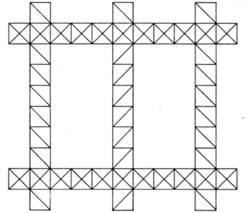
\includegraphics[scale=0.8]{"images/image013.jpg"}
\caption{‘ಗ್ರಿಡ್​ ಐರನ್​’ ಸಿಸ್ಟಮ್}\label{art11-fig1}
\end{figure}

ಮಳೆಗಾಲದ ಸಮಯವು, ಸರ್ವೇ ಕಾರ್ಯಾಚರಣೆಗೆ ದೀರ್ಘ ಸಮಯ ಹಿಡಿಯುವ, ಕಷ್ಟಕರವಾದ, ಆನಾರೋಗ್ಯಕರವಾದ ಕಾಲವಾಗಿತ್ತು. ಈ ಮಳೆಗಾಲದ ಅನಿವಾರ್ಯ ಕಾರ್ಯಾಚರಣೆಯನ್ನೂ ಸಹ ಎವರೆಸ್ಟ್​ರವರು ಬದಲಿಸಿದರು. ಹಗಲಿನ ಹೊತ್ತಿನಲ್ಲೂ\break ವೀಕ್ಷಣೆ ಮಾಡುವ ಹೀಲಿಯೋಟ್ರೋಪ್​ಗಳ ಉಪಯೋಗವನ್ನು ಜಾರಿಗೆ ತಂದರು.\break ಹೀಲಿಯೋಟ್ರೋಪ್​ ಎಂದರೆ, ಸೂರ್ಯನ ಬೆಳಕನ್ನು ಪ್ರತಿಫಲಿಸಿ, ಹೊಳೆಯುವ ವಸ್ತು. ರಾತ್ರಿ ಸಮಯದ ವೀಕ್ಷಣಾ ಕಾರ್ಯಕ್ಕೆ ಲಾಟೀನು ಮಾದರಿಯ ದೀಪವನ್ನು ಅಭಿವೃದ್ಧಿ ಪಡಿಸಿದರು. ಇದರಿಂದ ರಾತ್ರಿ ಸಮಯವೂ ಸೇರಿದಂತೆ, ಸರ್ವೇ ತಂಡಕ್ಕೆ ಅನುಕೂಲವಾದ ಆರೋಗ್ಯಕರ ಸಮಯದಲ್ಲಿಯೂ ವೀಕ್ಷಣಾ ಕಾರ್ಯ ಮಾಡಲು ಸಾಧ್ಯವಾಯಿತು. ಈ ಎಲ್ಲಾ ಸುಧಾರಣಾ ಕಾರಣಕ್ಕಾಗಿ ಸರ್ವೇ ಇತಿಹಾಸಕಾರರು, \enginline{1833} ರಿಂದ \enginline{1843} ರವರೆಗಿನ ಅವಧಿಯನ್ನು ‘ಎವರೆಸ್ಟ್​ರವರ ದಶಕ’ ಎಂದು ಕರೆದಿದ್ದಾರೆ.

ಎವರೆಸ್ಟ್​ರವರು ರಜಾದಲ್ಲಿದ್ದಾಗ, ಕೊಲ್ಕತ್ತಾ ಲಾಂಗಿಟ್ಯೂಡಿನಲ್​ ಸರಣಿಯ ಸರ್ವೇ ಕಾರ್ಯವನ್ನು ಜೋಸೆಫ್​ ಆಲೀವರ್​ ಎಂಬ ಇಂಗ್ಲೀಷ್​ ಅಧಿಕಾರಿ ಮಾಡಿದ್ದರು. ಈ ಸರಣಿಯು ಕಲ್ಯಾಣಪುರದಿಂದ ಆರಂಭವಾಗಿ ಕೊಲ್ಕತ್ತಾದಲ್ಲಿ ಕೊನೆಗೊಳ್ಳುತ್ತದೆ. ಎವರೆಸ್ಟ್​ರವರು ಇಂಗ್ಲೆಂಡಿನಿಂದ ಮರಳಿದ ತಕ್ಷಣ ಈ ಸರಣಿಯ ನಿಖರತೆಯ ಪರಿಶೀಲನೆಗಾಗಿ, ಕೊಲ್ಕತ್ತಾ ಬೇಸ್​ ಲೈನ್​ ಅಳತೆ ಮಾಡಲು ನಿರ್ಧರಿಸುತ್ತಾರೆ. ಆರೂವರೆ ಮೈಲು ಉದ್ದದ ಈ ಬೇಸ್​ಲೈನು, ಕೊಲ್ಕತ್ತಾ ಸರ್ಕಾರಿ ಗೃಹ ಮತ್ತು ಬರಾಕ್​ಪುರ ನಡುವಿನ ರಸ್ತೆಯಲ್ಲಿದೆ. ಈ ಬೇಸ್​ಲೈನಿನ ಎರಡೂ ತುದಿಗಳಲ್ಲಿ \enginline{75} ಅಡಿ ಎತ್ತರಕ್ಕೆ ಅದಕೆಂದೇ ನಿರ್ಮಿಸಿದ ಗೋಪುರಗಳು ಇವೆ. ಚಿತ್ರದ ಹಿನ್ನೆಲೆಯಲ್ಲಿ ಆ ಒಂದು ಗೋಪುರವನ್ನು ಗಮನಿಸಬಹುದು. ಅಳತೆ ಕಾರ್ಯವು ನವಂಬರ್​ \enginline{23}, \enginline{1831} ರಲ್ಲಿ ಆರಂಭವಾಗಿ, ಜನವರಿ \enginline{21}, \enginline{1832} ರಲ್ಲಿ ಮುಗಿಯುತ್ತದೆ. ಇದು ಭಾರತದಲ್ಲಿ, ಕಾಂಪೆನ್ಸೇಟಿಂಗ್​ ಬಾರ್​ ಬಳಸಿ ಮಾಡಿದ ಮೊದಲ ಬೇಸ್​ ಲೈನ್​ ಅಳತೆ ಕಾರ್ಯ.

ಲ್ಯಾಂಬಟನ್​ರವರ ಕಾಲದಲ್ಲಿ ಬೇಸ್​ ಲೈನ್​ ಅಳತೆಯನ್ನು ಸರಪಳಿ ಬಳಸಿ ಮಾಡಲಾಗುತ್ತಿತ್ತು. ಸರಪಳಿ ವಿಧಾನದಲ್ಲಿನ ಅನಾನುಕೂಲವೆಂದರೆ, ಇದರ ಕೊಂಡಿಗಳು ಬಳಸಿದಂತೆಲ್ಲಾ ಬೇಗ ಸವೆಯುತ್ತವೆ. ಸವೆದು ಉದ್ದದಲ್ಲಿ ಹಿಗ್ಗುತ್ತವೆ. ಅದರ ವಿವಿಧ ಭಾಗಗಳ ಉಷ್ಣತೆಯನ್ನು ನಿರ್ಧರಿಸುವುದೂ ಸಹ ಸುಲಭವಲ್ಲ. ಸರಪಳಿ ವಿಧಾನದಲ್ಲಿನ ಈ ನ್ಯೂನತೆಯ ಕಾರಣಕ್ಕೆ, ಐರಿಷ್​ ಸರ್ವೇಯ ಮುಖ್ಯಸ್ಥರಾದ ಕರ್ನಲ್​ ಕೋಲ್​ಬಿ ಯವರು ಕಾಂಪನ್​ಸೇಷನ್​ ಬಾರ್​ಗಳಿಂದ ಬೇಸ್​ ಲೈನ್​ ಅಳತೆ ಮಾಡುವ ಕ್ರಮವನ್ನು ಹೊಸದಾಗಿ ಆವಿಷ್ಕಾರ ಮಾಡಿದ್ದರು. ಕಾಂಪನ್​ಸೇಷನ್​ ಬಾರ್​ ಅಂದರೆ ಮೂಲತಹ ಅದು ಅಳತೆಗೋಲು. ವಿವಿಧ ಲೋಹಗಳು ಉಷ್ಣತೆಗೆ ವಿವಿಧ ರೀತಿಯಾಗಿ ಹಿಗ್ಗುತ್ತವೆ. ಈ ವಿಶೇಷ ಗುಣವನ್ನೇ ಬಳಸಿಕೊಂಡು, ಉಷ್ಣತೆಯ ಆ ಪರಿಣಾಮವನ್ನು ಪೂರ್ಣವಾಗಿ ಸರಿದೂಗಿಸುವ ತತ್ವವನ್ನು ಆಧರಿಸಿದೆ ಈ ವಿಧಾನ. ಉಷ್ಣತೆಯ ವ್ಯತ್ಯಾಸದಿಂದ ಹಿಗ್ಗಿದ ಅಥವಾ ಕುಗ್ಗಿದ ಪ್ರಮಾಣವು ಕಾಂಪನ್​ಸೇಟ್​ ಆಗುವಂತೆ ಕಾಂಪನ್​ಸೇಷನ್​ ಬಾರ್​ಗಳನ್ನು ವಿಶೇಷವಾಗಿ ರಚಿಸಲಾಗಿರುತ್ತದೆ. ಎವರೆಸ್ಟ್​ ರವರು ರಜೆಯ ಮೇಲೆ ಇಂಗ್ಲೆಂಡಿನಲ್ಲಿದ್ದಾಗ, ಅಲ್ಲಿ ಬೇಸ್​ ಲೈನ್​ ಅಳತೆಗೆ ಕಾಂಪನ್​ಸೇಷನ್​ ಬಾರ್ಸ್​ ಬಳಕೆಯನ್ನು ನೋಡಿದ್ದರು. ಭಾರತಕ್ಕೆ ಹೊರಡುವ ಮೊದಲು ಕಾಂಪನ್​ಸೇಷನ್​ ಬಾರ್​ಗಳನ್ನು ಲಾರ್ಡ್ಸ್ ಕ್ರಿಕೆಟ್​ ಮೈಧಾನದಲ್ಲಿ ಪರೀಕ್ಷಾರ್ಥವಾಗಿ ಅವರು ಸ್ವತಃ ಬಳಸಿ ನೋಡಿದ್ದರು.

\begin{figure}[!hbtp]
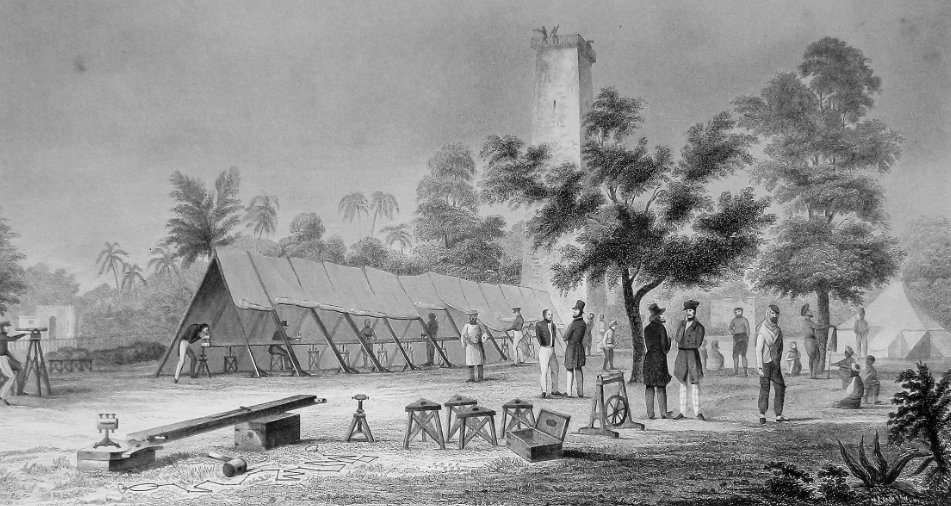
\includegraphics[scale=0.6]{"images/image014.jpg"}
\caption{ಕೊಲ್ಕತ್ತಾ ಬೇಸ್​ ಲೈನ್​ ಅಳತೆ ಕಾರ್ಯ}\label{art11-fig2}
\end{figure}

\newpage

ಬೇಸ್​ ಲೈನ್​ ಅಳತೆ ಕಾರ್ಯವು ಸರಳವಾದುದಲ್ಲ. ಅದು ಬಹು ಸಂಕೀರ್ಣ ಕಾರ್ಯ. ಬಹಳಷ್ಟು ವಿಧಿ ವಿಧಾನಗಳನ್ನು ಅನುಸರಿಸಬೇಕಾಗುತ್ತದೆ. ಅದರ ಎರಡು ಅಂತಿಮ ಬಿಂದುಗಳ ನಡುವಿನ ನೆಲವನ್ನು ಕ್ಲಿಯರ್​ ಮಾಡಿ, ನೇರಗೊಳಿಸಿ, ಮಟ್ಟ ಮಾಡಬೇಕು. ತ್ರಿಪಾದಿಗಳನ್ನು ಸ್ಥಾಪಿಸಿ, ಅವುಗಳ ಮೇಲೆ ಉದ್ದನೆಯ ತೆರೆದ ಪೆಟ್ಟಿಗೆ, ಕಾಫರ್​ಗಳಅನ್ನಿಟ್ಟು, ತ್ರಿಪಾದಿಗಳಿಂದ ಅವುಗಳನ್ನು ಮಟ್ಟಮಾಡಬೇಕು. ಈಗ ಕಾಂಪನ್ಸೇಷನ್​ ಬಾರ್​ಗಳನ್ನು ಕಾಫರ್​ಗಳಲ್ಲಿ ಇರಿಸಬೇಕು. ಮೇಲೆ ಬಿಸಿಲು ಬೀಳದ ಹಾಗೆ, ನೆರಳು ಬೀಳುವ ಹಾಗೆ, ಚಾವಣಿಯನ್ನು ಹಾಕಬೇಕು. ಈ ವಿವರಗಳನ್ನು ಬೇಸ್​ ಲೈನ್​ ಅಳತೆ ಕಾರ್ಯದ ಚಿತ್ರದಲ್ಲಿ ಗಮನಿಸಬಹುದು. ಎರಡು ಬಾರ್​ಗಳ ತುದಿಗಳನ್ನು, ಮೈಕ್ರೊಸ್ಕೋಪನ್ನು ಬಳಸಿ ಒಂದು ಕೂದಲೆಳೆಯ ಅಂತರವೂ ವ್ಯತ್ಯಾಸಗೊಳ್ಳದಂತೆ, ಒಂದರ ಪಕ್ಕ ಒಂದನ್ನು ಕೂರಿಸಬೇಕು. ಬೇಸ್​ ಲೈನ್​ ಅಳತೆಯನ್ನು ಚೈನ್​ ಬಳಸಿ ಮಾಡಲಾಗುತಿದ್ದರೆ, ಆಗ ಅಳತೆಗೆ ಬಳಸುತ್ತಿರುವ ಚೈನನ್ನು ಸ್ಟ್ಯಾಂಡರ್ಡ್ ಚೈನ್​ನ ಜೊತೆ, ಪ್ರತಿ ಸಲವೂ ಹೋಲಿಸಿ ನೋಡಬೇಕು. ಸರಪಳಿ ಎಳೆತವನ್ನು, ಪ್ರತಿ ಸಲ \enginline{19} ಪೌಂಡ್​ ಭಾರದಲ್ಲಿಯೇ ಸಮಾನವಾಗಿ ಎಳೆಯಬೇಕು. ಅಳತೆಯ ಆರಂಭದಲ್ಲಿ ಮತ್ತು ಕೊನೆಯಲ್ಲಿ ಥರ್ಮಾಮೀಟರ್​ನಿಂದ ತಾಪವನ್ನು ಓದಬೇಕು. ಉಷ್ಣತೆಯಿಂದ ಹಿಗ್ಗುವಿಕೆ ಮತ್ತು ಕುಗ್ಗುವಿಕೆಯು, ಪ್ರತಿ ಫ್ಯಾರೆನ್​ಹೀಟ್​ ವ್ಯತ್ಯಾಸಕ್ಕೆ, \enginline{100} ಅಡಿಯ ಸರಪಳಿಯಲ್ಲಿ, \enginline{0.0075} ಇಂಚ್​ ಇರುತ್ತದೆ. ಅಳತೆಗೆ, ಉಷ್ಣತೆಯ ಈ ತಿದ್ದುಪಡಿಯನ್ನು ಅಳವಡಿಸಿಕೊಳ್ಳಬೇಕು. ಭೂಮಿಯ ವಕ್ರತೆಗೂ ಸಹ ತಿದ್ದುಪಡಿಯನ್ನು ಅಳವಡಿಸಿ ಕೊಳ್ಳಬೇಕು. ಅಂದರೆ, ಅಳೆದ ಬೇಸ್​ ಲೈನ್​ ಒಟ್ಟು ಉದ್ದವನ್ನು, ಸರಾಸರಿ ಸಮುದ್ರ ಮಟ್ಟಕ್ಕೆ ಇಳಿಸಿ, ಲೆಕ್ಕಾಚಾರ ಮಾಡಬೇಕು. ಬೇಸ್​ ಲೈನ್​ ಅಳತೆ ಕಾರ್ಯಕ್ಕೆ ಗಣಿತ, ಜಿಯೊಡೆಸಿ, ಫಿಸಿಕ್ಸ್​ ನಂತಹ ಮೂಲ ವಿಜ್ಞಾನದ ಅರಿವು ಇರಬೇಕು. ಈ ಎಲ್ಲಾ ಜ್ಞಾನವನ್ನು ಕ್ಷೇತ್ರ ಕಾರ್ಯದಲ್ಲಿ ಅನ್ವಯಿಸಿಕೊಳ್ಳುವ ಕೌಶಲ್ಯವಿರಬೇಕು.

ಉತ್ತರಾಂಚಲದ ಮಸೂರಿಯಲ್ಲಿ ಎವರೆಸ್ಟ್​ರವರು ಒಂದು ಎಸ್ಟೇಟನ್ನು ಕೊಂಡರು. ಅಲ್ಲಿ ಹೊಸದಾಗಿ ತಮ್ಮ ಸರ್ವೇ ಕೇಂದ್ರ ಸ್ಥಾನವನ್ನು ಸ್ಥಾಪಿಸಿದರು. ಮುಂದೆ ಈ ಕೇಂದ್ರದಿಂದಲೇ ಎಲ್ಲಾ ಕಾರ್ಯಗಳೂ ನಡೆಯುವಂತೆ ಮಾಡಿದರು. ಹಿಮಾಲಯದ ಅದ್ಭುತ ದೃಶ್ಯಾವಳಿ, ಪರ್ವತಗಳ ಶ್ರೇಣಿ, ಅದ್ಬುತ ಎತ್ತರ ಇವುಗಳತ್ತ ಎವರೆಸ್ಟ್​ರವರು, ತಮ್ಮ ಗಮನವನ್ನು ನೀಡಿದರು. ಹೀಗೆ ಗ್ರೇಟ್​ ಆರ್ಕ್ ಅಳತೆ ಕಾರ್ಯವು ಹಿಮಾಲಯದ ತಪ್ಪಲು ತಲುಪಿತು.

ಕರ್ನಲ್​ ಮೆಕೆಂಜೀ, ಎವರೆಸ್ಟ್​ರಂಥವರು ಮುಖ್ಯಸ್ಥರಾಗಿದ್ದ ಸರ್ವೇ ಆಫ್​ ಇಂಡಿಯಾದ ಕೇಂದ್ರ ಕಛೇರಿ ಈಗ ಸ್ವತಂತ್ರ ಭಾರತದಲ್ಲಿ ಇರುವುದು ಡೆಹರಾಡೂನ್​ನಲ್ಲಿ. ಈ ಮೊದಲು ಕೋಲ್ಕತ್ತಾದಲ್ಲಿದ್ದ ಸರ್ವೇ ಕೇಂದ್ರವನ್ನು ಇಷ್ಟೊಂದು ಹಿತಕರ ತಾಣದಲ್ಲಿ ಸ್ಥಾಪಿಸಿದ ಕೀರ್ತಿ ಎವರೆಸ್ಟ್​ ಅವರಿಗೆ ಸಲ್ಲುತ್ತದೆ. ಸರ್ವೇಯರ್​ ಜನರಲ್​ ಮತ್ತು ಟ್ರಿಗನಮಿಟ್ರಿಕಲ್​ ಸರ್ವೇಯ ಸೂಪರಿಂಟೆಂಡೆಂಟ್​ ಸ್ಥಾನಗಳ ದ್ವಿಪಾತ್ರದಲ್ಲಿ, ಈ ಎರಡೂ ಹುದ್ದೆಯ ಜವಾಬ್ದಾರಿಯನ್ನು ನಿರ್ವಹಿಸಲು ಕೊಲ್ಕತ್ತಾದಿಂದ ಸರ್ವೇ ಕೇಂದ್ರವನ್ನು ಡೆಹರಾಡೂನಿಗೆ ಸ್ಥಳಾಂತರಿಸುವುದು ಅಗತ್ಯವೆಂದು ಎವರೆಸ್ಟ್​ರವರು ಪಟ್ಟು ಹಿಡಿದರು. ಜೊತೆಗೆ ಆರೋಗ್ಯಕರ ಹಿತಕರ ಜಾಗದಲ್ಲಿ ಮುಖ್ಯ ಕೇಂದ್ರ ಸ್ಥಾನ ಇರಬೇಕೆಂದು ಹೇಳಿದರು. ಆದರೆ, ಇಡೀ ಸರ್ವೇ ಕೇಂದ್ರದ ಪೂರ್ಣ ಸ್ಥಳಾಂತರವನ್ನು ಸರ್ಕಾರ ಒಪ್ಪುವುದಿಲ್ಲ. ಇದರಿಂದ, ಕಂಪ್ಯುಟೇಶನ್​, ಮ್ಯಾಪಿಂಗ್​, ಆಡಳಿತಾತ್ಮಕ ಘಟಕಗಳು ಕಲ್ಕತ್ತಾದಲ್ಲಿಯೇ ಉಳಿಯುವಂತಾಯಿತು.

ಗ್ರೇಟ್​ ಆರ್ಕ್ನ ಅತ್ಯಂತ ಉತ್ತರ ಭಾಗದಲ್ಲಿ ಡೆಹರಾಡೂನಿನ ಬೇಸ್​ ಲೈನ್​ ಇದೆ. ಡೆಹರಾಡೂನ್​ನ ಈ ಬೇಸ್​ ಲೈನ್​ನ ಅಳತೆ ಕಾರ್ಯವನ್ನು ಡಿಸೆಂಬರ್​ \enginline{1834} ರಲ್ಲಿ ಪ್ರಾರಂಭಿಸಲಾಯಿತು. ಸವಾಲಿಕ್​ ಬೆಟ್ಟ ಮತ್ತು ಹಿಮಾಲಯ ನಡುವಿನ ಸುಂದರ ಕಣಿವೆಯೇ ಡೆಹರಾಡೂನ್​ ಇರುವ ಸ್ಥಳ. ಸರಾಸರಿ ಸಮುದ್ರ ಮಟ್ಟದಿಂದ ಸುಮಾರು \enginline{2000} ಅಡಿ ಎತ್ತರ ಪ್ರದೇಶ. ಈ ಬೇಸ್​ ಲೈನ್​ನ ಅಳತೆ ಕಾರ್ಯವನ್ನು ಡಿಸೆಂಬರ್​ \enginline{1} ರಂದು ಪ್ರಾರಂಭಿಸಲಾಯಿತು. ಮಾರ್ಚ್ \enginline{28}, \enginline{1835} ರಲ್ಲಿ ಈ ಬೇಸ್​ ಲೈನ್​ನ ಅಳತೆ ಕಾರ್ಯವು ಮುಗಿಯಿತು. \enginline{1838} ರಲ್ಲಿ ಕ್ಯಾಪ್ಟನ್​ ವಾಗ್​ರವರನ್ನು ಟ್ರಫ್​ಟನ್​ ಕಂಪನಿಯ ಹೊಸ ಥಿಯಡೊಲೈಟ್​ನಿಂದ ಕೋನಗಳ ಮರು ಅಳತೆಗೆ ಕಳಿಸಲಾಯಿತು. ವಾಗ್​ರವರು ಅದ್ಭುತ ನಿಖರತೆಯಲ್ಲಿ ಗ್ರೇಟ್​ ಆರ್ಕ್ ಟ್ರ್ಯಾಂಗ್ಯುಲೇಶನ್​ ಸರಣಿಯ ಅಳತೆಯನ್ನು ಪೂರೈಸುತ್ತಾರೆ. ಸಿರೋಂಜ್​ ಬೇಸ್​ನಿಂದ ಮುಂದುವರೆದ ಟ್ರ್ಯಾಂಗ್ಯುಲೇಶನ್​ನಿಂದ ದೊರೆತ ಅಳತೆಗೂ, ಡೆಹರಾಡೂನ್​ನಲ್ಲಿ ನೇರವಾಗಿ ಮಾಡಿದ ಅಳತೆಗೂ ವ್ಯತ್ಯಾಸವು ಕೇವಲ \enginline{7.2} ಅಂಗುಲ ಕಂಡುಬಂತು.

ಎವರೆಸ್ಟ್​ ಅವರಿಗೆ ಮತ್ತೊಮ್ಮೆ ಅನಾರೋಗ್ಯ ಕಾಡಿತು. ಸಂಧಿವಾತ, ಮೂಳೆಗಳಲ್ಲಿ ಭಯಾನಕ ನೋವು, ಜ್ವರ, ಹಸಿವು ಇಲ್ಲದಿರುವಿಕೆ, ಅಜೀರ್ಣ, ಹೊಟ್ಟೆಯಲ್ಲಿ ಅಶಕ್ತಿ ಈ ತೊಂದರೆಗಳು ಉಂಟಾದವು. ಒಟ್ಟಿನಲ್ಲಿ ಎವರೆಸ್ಟ್​ರವರಿಗೆ ಟೆಂಟಿನ ಸೆರೆವಾಸ ಗತಿಯಾಯಿತು. ಈ ಸಮಯದಲ್ಲಿ ಅವರ ನೆಚ್ಚಿನ ಶಿಷ್ಯ ಆಂಡ್ರ್ಯೂ ವಾಗ್​ರವರು ಸಮರ್ಥವಾಗಿ ಬೇಸ್​ಲೈನ್​ ಅಳತೆ ಕಾರ್ಯವನ್ನು ನಿರ್ವಹಿಸಿದರು. ಸಿರೋಂಜ್​ ಮತ್ತು ಡೆಹರಾಡೂನ್​ ಬೇಸ್​, ಇವುಗಳ ನಡುವೆ \enginline{450} ಮೈಲುಗಳ ಅಂತರವಿದೆ. ಮತ್ತು \enginline{86} ಪ್ರಧಾನ ತ್ರಿಭುಜಗಳಿವೆ. ಟ್ರಾಂಗ್ಯುಲೇಷನ್​ ಕಾರ್ಯ ಇಷ್ಟೊಂದು ದೂರ ಕ್ರಮಿಸಿ ಬಂದಿದೆ. ಸಿರೋಂಜ್​ ಬೇಸ್​ ಲೈನ್​ ಏಳುಕಾಲು ಮೈಲು ಉದ್ದವಿದೆ. ಅದರ ನಿಖರತೆಯನ್ನು ಅಳೆದು ನೋಡಿದಾಗ ಕೇವಲ \enginline{6.395} ಅಂಗುಲದಷ್ಟು ವ್ಯತ್ಯಾಸ ಬಂದಿತು. ನಿಜವಾಗಿ ತೃಪ್ತಿಕರ ನಿಖರತೆಯೇ. ಇದು ಇಂಚು ನಿಖರತೆಯ ವೈಜ್ಞಾನಿಕ ಮಹಾ ಕಾರ್ಯಕ್ಕೆ ಸಾಕ್ಷಿ.

ಎವರೆಸ್ಟ್​ರವರಿಗೆ ಅವರ ಕಣ್ಣಿನ ದೃಷ್ಟಿ ಮಂಜಾಗುತ್ತಾ ಬಂತು. ನೆನಪಿನ ಶಕ್ತಿಯೂ ಕುಂದಿತ್ತು. ಕಾಯಿಲೆ ಉಲ್ಬಣಿಸಿ, ಭೂತ ಹಿಡಿದವರಂತೆ ಭ್ರಮಣೆಗೆ ಒಳಗಾಗಿದ್ದರು. ನಿದ್ದೆಯಲ್ಲೂ ಆ ಭ್ರಮಣೆಯು ಅವರನ್ನು ಕಾಡುತ್ತಿತ್ತು. ಎಚ್ಚರ ಸ್ಥಿತಿಯಲ್ಲೂ ಕಾಡುತ್ತಿತ್ತು. ಅವರೇ ಹೇಳಿಕೊಂಡಂತೆ “ಖಂಡಿತಾವಾಗಿಯೂ ಇಲ್ಲಿ ನಿಜವಾಗಿಯೂ ಹುಚ್ಚು ಹಿಡಿಯುತ್ತಿದೆ. ಉತ್ತಮ ಹವೆಯ ಪರಿಸರಕ್ಕೆ ಬರದಿದ್ದರೆ ಮತ್ತು ಪ್ರತಿಜ್ಞೆಗೈದ ಕೈಗೊಂಡ ಕಾರ್ಯವು ಇಲ್ಲದೇ ಹೋಗಿದ್ದರೆ....”. ಅವರಿಗೆ ಈ ಉತ್ತಮ ಹವೆಯ ಪರಿಸರವೆಂದರೆ, ಅದು ಡೆಹರಾಡೂನ್​ ಹಾಥಿಪಾನ್​ ಗೃಹಕಛೇರಿ. ಆ ಸಮಯಕ್ಕೆ ಎವರೆಸ್ಟ್​ರವರ ಕ್ಷೇತ್ರ ಕಾರ್ಯದ ದಿನಗಳು ಹೆಚ್ಚು ಕಡಿಮೆ ಮುಗಿದಿದ್ದವು. ಖಗೋಳ ವೀಕ್ಷಣೆ, ಕಂಪ್ಯೂಟಿಂಗ್​ ಕಾರ್ಯ ಇವುಗಳ ಮೇಲ್ವಿಚಾರಣೆಗಷ್ಟೇ ಗಮನಕೊಡಲು ಅವರು ನಿರ್ಧರಿಸಿದರು. ಅವರ ಸಮರ್ಥ ನಂಬಿಗಸ್ಥ ಸಹಾಯಕ ಆಂಡ್ರ್ಯೂ ವಾಗ್​ರವರು ಅಂತಿಮ ಹಂತದ ಉಳಿದ ಟ್ರೈಯಾಂಗ್ಯುಲೇಷನ್ನಿನ ಜವಾಬ್ದಾರಿಯನ್ನು ತೆಗೆದುಕೊಂಡರು.

ಈ \enginline{1836}ರ ಅವಧಿಯಲ್ಲಿ ಎವರೆಸ್ಟ್​ರವರ ಆರೋಗ್ಯವು ಮತ್ತಷ್ಟು ಹದಗೆಟ್ಟಿತು. ಅವರು ಬದುಕುಳಿಯುವುದೇ ಯಾರಿಗೂ ನಂಬಿಕೆ ಇರಲಿಲ್ಲ. ಎವರೆಸ್ಟ್​ರವರು ತಮ್ಮ ಅನಾರೋಗ್ಯದಿಂದ ಏನಾದರೂ ತೀರಿಕೊಂಡುಬಿಟ್ಟರೆ, ಆಗ ಟ್ರ್ಯಾಂಗ್ಯುಲೇಶನ್​ ಕಾರ್ಯಕ್ಕೆ ಅದರಿಂದ ಅಡಚಣೆಯಾಗಬಾರದೆಂದು, ಸರಕಾರವು ಎವರೆಸ್ಟ್​ರವರ ಮರಣದ ನಂತರದ ಸಂದರ್ಭಕ್ಕೆಂದು ಮೇಜರ್​ ಜೆರ್ವಿನ್​ರವರನ್ನು ಮುಂದಾಗಿಯೇ ಅವರ ಉತ್ತರಾಧಿಕಾರಿಯನ್ನಾಗಿ ನೇಮಿಸಿದ ಘಟನೆಯೂ ನಡೆಯಿತು. ಆದರೆ, ಸರಕಾರವೇ ನಿರೀಕ್ಷಿಸಿದ್ದ ದುರ್ಘಟನೆಯೇನೂ ಎವರೆಸ್ಟ್​\break ರವರಿಗೆ ಸಂಭವಿಸುವುದಿಲ್ಲ. ಈ ಕಾರಣದಿಂದ ಮೇಜರ್​ ಜೆರ್ವಿನ್​ರವರು ಟ್ರಿಗನಮಿಟ್ರಿಕಲ್​ ಸರ್ವೇ ಕಾರ್ಯಕ್ಕೆ ಬರುವ ಸಂದರ್ಭ ಬರಲಿಲ್ಲ.

ನಾವಿರುವ ಈ ಭೂಮಿಯ ನಿಖರವಾದ ರೂಪ ಆಕಾರ ಏನೆಂಬುದನ್ನು ಕಂಡುಹಿಡಿಯುವುದು ಮಾನವ ವಿಜ್ಞಾನಕ್ಕೆ ನಿಜವಾದ ಮೂಲ ಸವಾಲು. ಗ್ರೇಟ್​ ಆರ್ಕ್ ಸರ್ವೇ ಕಾರ್ಯಕ್ಕೆ ಮ್ಯಾಪಿಂಗ್​ ಮಹತ್ವದ ಜೊತೆಗೆ, ಭೂವಿಜ್ಞಾನದ ಮಹತ್ವವೂ ಇದೆಯೆಂದು ನೋಡಿದ್ದೇವೆ. ನಮ್ಮ ಈ ಭೂಮಿಯ ನಿಖರವಾದ ರೂಪ, ಆಕಾರ ಎಂತಹದ್ದು ಎಂದು ಗಣಿತಾತ್ಮಕವಾಗಿ ಸಿದ್ಧಪಡಿಸುವ ನಿಕಟ ತಾಜಾ ಪ್ರಾಯೋಗಿಕ ಫಲಿತಾಂಶವನ್ನು ಎವರೆಸ್ಟ್​ರವರಿಗೆ ಅವರ ಗ್ರೇಟ್​ ಆರ್ಕ್ ಸರ್ವೇ ಕಾರ್ಯ ನೀಡಿತ್ತು. ಅದು ಹೇಗೆಂದರೆ, ಗ್ರೇಟ್​ ಆರ್ಕ್ ಮೇಲಿನ ಬೀದರ್​, ಸೀರೋಂಜ್​, ಕಲ್ಯಾಣಗಳ ಟ್ಯಾಂಗ್ಯುಲೇಷನ್​ ಪಾಯಿಂಟ್​ಗಳ ಮೇಲಿನ ಅಕ್ಷಾಂಶವನ್ನು ಸೆಕೆಂಡಿನ ಸಹಸ್ರಾಂಶ ಭಾಗದ ನಿಖರತೆಯ ಮಟ್ಟಕ್ಕೆ, ಇಂತಿಷ್ಟು ಡಿಗ್ರಿ ಮಿನಿಟ್​ ಸೆಕೆಂಡ್​ ಎಂದು ಲೆಕ್ಕಾಚಾರದಿಂದ ಕಂಡುಕೊಳ್ಳಲಾಗಿದೆ. ಈ ಮೌಲ್ಯವನ್ನು ಎವರೆಸ್ಟ್​ ಮತ್ತು ಆಂಡ್ರ್ಯೂ ವಾಗ್​ರವರು ಸಾವಿರಾರು ಖಗೋಳ ವೀಕ್ಷಣೆ ಮಾಡಿ ಕೋನ ಓದುವುದರ ಮೂಲಕ ಕಂಡುಕೊಂಡಿದ್ದರು. ಅವರು ಖಗೋಳ ವೀಕ್ಷಣೆಯಿಂದ ಕಂಡುಕೊಂಡ ಫಲಿತಾಂಶವೇ, ಗ್ರೇಟ್​ ಆರ್ಕ್ ಮೇಲಿನ ಆ ಬಿಂದುಗಳ ನಡುವಿನ ಕೋನೀಯ ಅಂತರ. ಅದೇ ಬಿಂದುಗಳ ನಡುವಿನ ನೈಜ ದೂರವನ್ನು ಸಹ ಕಾರ್ಯರೂಪದಲ್ಲಿ, ಟ್ರೈಯಾಂಗ್ಯುಲೇಷನ್​ ವಿಧಾನದಿಂದ ಅಳೆಯಲಾಗಿದೆ. ಆರ್ಕ್ ಮೇಲಿನ ಆ ಬಿಂದುಗಳ ನಡುವಿನ ಕೋನ ಮತ್ತು ದೂರ ತಿಳಿದಿದೆ. ಈಗ ಗಣಿತ ಸೂತ್ರ ಬಳಸಿ ಸುಲಭವಾಗಿ ಆರ್ಕ್ನ ರೇಡಿಯಸ್ಸನ್ನು ಲೆಕ್ಕಚಾರ ಮಾಡಬಹುದು. ಆರ್ಕ್ನ ರೇಡಿಯಸ್​ ಅಂದರೆ ಅದು ಭೂಮಿಯ ರೇಡಿಯಸ್​. ಹೀಗೆ ಭೂಮಿಯ ರೇಡಿಯಸ್​ ಹಾಗೂ ಸುತ್ತಳತೆಯನ್ನು ನೀಡಿದ ಗ್ರೇಟ್​ ಆರ್ಕ್ ಅಳತೆ ಕಾರ್ಯ ಆರಂಭಿಸಿದ ಮಹನೀಯರ ಕಾರ್ಯವು ನಿಜವಾಗಿಯೂ ವೈಜ್ಞಾನಿಕ ಮಹತ್ವದ್ದು.

ಭೂಮಿಯು ಸಮಭಾಜಕದಲ್ಲಿ ಉಬ್ಬಿದೆ. ಧೃವ ಪ್ರದೇಶದಲ್ಲಿ ಚಪ್ಪಟೆಯಾಗಿದೆ. ಸಮಭಾಜಕ ತ್ರಿಜ್ಯವು, ಧೃವೀಯ ತ್ರಿಜ್ಯಕ್ಕಿಂತ \enginline{67260} ಅಡಿ ಹೆಚ್ಚಾಗಿದೆ ಎಂದು ಎವರೆಸ್ಟ್​ರವರು ತಮ್ಮ ಟ್ರಿಗನಮಿಟ್ರಿಕಲ್​ ಸರ್ವೇಯ ನೂತನ ಪ್ರಾಯೋಗಿಕವಾದ ಲೆಕ್ಕಾಚಾರದಿಂದ ತೋರಿಸಿಕೊಟ್ಟರು. ಭೂವಿಜ್ಞಾನ ಕ್ಷೇತ್ರದ ಲೆಕ್ಕಾಚಾರದಲ್ಲಿ ತೊಡಗಿಸಿಕೊಂಡ ಯುರೋಪಿನ ಘನ ವಿದ್ವಾಂಸರನ್ನು ಚಕಿತಗೊಳಿಸುವ ಮಹತ್ಕಾರ್ಯ ಇದು.

ಸರ್ಕಾರಕ್ಕಾಗಲೀ ಜನಕ್ಕಾಗಲೀ ಮ್ಯಾಪಷ್ಟೇ ಬೇಕು. ಜತೆಗೆ ಮ್ಯಾಪಿನ ಟ್ರಿಗನಮಿಟ್ರಿಕಲ್​ ಸ್ಟೇಷನ್ನಿನ ಕೋಆರ್ಡಿನೇಟ್​ಗಳು ಸಾಕು. ಆದರೆ ನಿಖರ ಡೀಟೈಲು ಸರ್ವೇ ಮ್ಯಾಪಿಂಗ್​ ಕಾರ್ಯಕ್ಕೆ ಫ್ರೇಮ್ವರ್ಕ್ ಕಾರ್ಯ ಮೊದಲು ಆಗಬೇಕು. ಗಣಿತದ ಗಟ್ಟಿ ನೆಲಗಟ್ಟಿನ ಮೇಲೆ ನಿಂತ ಆ ಫ್ರೇಮ್ವರ್ಕಿನ ಮೇಲೆ ಡೀಟೈಲು ಮ್ಯಾಪನ್ನು ಕೂರಿಸಬಹುದು. ಸರಕಾರಕ್ಕೆ ಮತ್ತು ಉಳಿದವರಿಗೆ ಆ ಫ್ರೇಮ್ವರ್ಕಿನ ಮಿಕ್ಕಿದ್ದೆಲ್ಲ ವಿಷಯಗಳು ಅರ್ಥವಾಗದ ನಿಗೂಢ ಕ್ಲಿಷ್ಠಕರ ವಿಚಾರ. ಸಾವಿರಾರು ಪುಟಗಳ ಎವರೆಸ್ಟ್​ರವರ ವರದಿಯಲ್ಲಿ ಬರಿಯ ಅಂಕಿ ಸಂಖ್ಯೆ, ವಕ್ರೀಭವನ ಸಮಸ್ಯೆ, ಪ್ಲಮೆಟ್​ ಲೈನು ಗುರುತ್ವ ಭಾರದಿಂದ ತನ್ನ ನೇರದಿಂದ ಹೊರ ಬಾಗುವಿಕೆಯ ಸಮಸ್ಯೆ, ಖಗೋಳ ವೀಕ್ಷಣೆ ವಿವರಣೆಗಳು, ಪುಟ ಉದ್ದದ ಫಾರ್ಮುಲಾಗಳು ಇವುಗಳೇ ಸಿಗುತ್ತವೆ. ಆಗ ಲೆಕ್ಕಾಚಾರಕ್ಕೆ ಕ್ಯಾಲುಕಲೇಟರು, ಕಂಪ್ಯೂಟರು, ಪ್ರೋಗ್ರಾಮ್ಗಳು ಇರದ ದಿನಗಳು. ಲೆಕ್ಕಾಚಾರಕ್ಕೆ ಲಾಗರಿದಮ್ ಟೇಬಲ್ಲುಗಳೇ ಗತಿ, ಅಂತಹ ಕಾಲ ಅದು.

\enginline{1802}ರಲ್ಲಿ ಆರಂಭವಾದ ಗ್ರೇಟ್​ ಆರ್ಕ್ \enginline{1843}ರಲ್ಲಿ ಉತ್ತರದ ಡೆಹರಾಡೂನಿನಲ್ಲಿ ಮುಕ್ತಾಯ ಹಂತ ತಲುಪಿತು. ಎವರೆಸ್ಟ್​ರವರು ತಾವು ನಿವೃತ್ತರಾಗುವ ಮೊದಲು, ಅವರ ಮುಖ್ಯ ಸಹಾಯಕರಾಗಿದ್ದ ಲೆಫ್ಟಿನೆಂಟ್​ ಆಂಡ್ರ್ಯೂ ಸ್ಕಾಟ್​ ವಾಗ್​ ರವರನ್ನು ತಮ್ಮ ಉತ್ತರಾಧಿಕಾರಿಯನ್ನಾಗಿ ನೇಮಿಸಬೇಕೆಂದು ಸರಕಾರಕ್ಕೆ ಶಿಫಾರಸು ಮಾಡಿದ್ದರು. ಆಂಡ್ರ್ಯೂ ವಾಗ್​ರವರು ಸಹ ಇಲಾಖೆಯ ಎಲ್ಲಾ ಅಧಿಕಾರಿಗಳ ಗೌರವಾದರಗಳಿಗೆ ಪಾತ್ರರಾದ ಹಾಗು ತಾಂತ್ರಿಕ ನೈಪುಣ್ಯ ಹೊಂದಿದ್ದ, ಸಮರ್ಥ ವ್ಯಕ್ತಿಯಾಗಿದ್ದರು. \enginline{1843} ರಲ್ಲಿ, ಎವರೆಸ್ಟ್​ರವರು ತಮ್ಮ ನಿವೃತ್ತಿಯನ್ನು ಪಡೆದು ಊರಿಗೆ ಮರಳಿದರು. ಎವರೆಸ್ಟ್​ರವರು ಇಚ್ಚಿಸಿದಂತೆ, ಲೆಫ್ಟಿನೆಂಟ್​ ಆಂಡ್ರ್ಯೂ ವಾಗ್​ರವರು ಅವರ ಉತ್ತರಾಧಿಕಾರಿಯಾಗಿ, ಟ್ರಿಗನಮಿಟ್ರಿಕಲ್​ ಸರ್ವೇಯ ಮುಖ್ಯಸ್ಥರಾದರು.

ಗ್ರೇಟ್​ ಆರ್ಕ್ನ ಪಿತಾಮಹ ಲ್ಯಾಂಬ್​ಟನ್​ರವರು ತಮ್ಮ ವೃತ್ತಿ ಬದುಕಿನಲ್ಲಿರುವಾಗಲೇ, ಗ್ರೇಟ್​ ಆರ್ಕ್ನ ಮೇಲೆಯೇ ಮಡಿದು ಅಮರರಾದರು. ಎವರೆಸ್ಟ್​ರವರು ತೀವ್ರ ಅನಾರೋಗ್ಯ ಪೀಡಿತರಾಗಿ, ಕೆಲಸದಲ್ಲಿ ಮುಂದುವರೆಯಲಾಗದೇ ಮಧ್ಯದಲ್ಲಿಯೇ ನಿವೃತ್ತರಾಗಿ, ಊರಿಗೆ ವಾಪಾಸಾದರು. ಬೆಟ್ಟ, ಬಂಡೆ, ದುರ್ಗ, ಗೋಪುರ ಇವುಗಳ ಮೇಲೆ ಅವರಿಬ್ಬರೂ ಸ್ಥಾಪಿಸಿದ ಜಿಟಿಎಸ್​ ಸ್ಟೇಷನ್​ಗಳು ಇಂದು ಎರಡು ಶತಮಾನಗಳ ನಂತರವೂ ಸಹ ಇವೆ. ಟ್ರ್ಯಾಂಗ್ಯುಲೇಷನ್​ ಜಾಲದ ಉದ್ದಗಲಕ್ಕೂ ಅವು ಮಿನುಗಿ ಮಿಂಚಿ ತಮ್ಮ ಉದ್ದೇಶವನ್ನು ಸಾರ್ಥಕಗೊಳಿಸಿವೆ. ಟೋಪೋಗ್ರಫಿಕಲ್​ ಸರ್ವೇ, ಕೆಡಸ್ಟ್ರಲ್​ ಸರ್ವೇಗೆ ಇಂದಿನವರೆಗೂ ಅವುಗಳು ಆಧಾರಸ್ಥಂಭಗಳಾಗಿವೆ. ಆದರೆ ಈಗ ಕಾಲನ ಹೊಡೆತಕ್ಕೆ ಸಿಕ್ಕಿ, ನಶಿಸಿ ಮರೆಯಾಗುತ್ತಲಿವೆ. ಇಂತಹ ಟ್ರ್ಯಾಂಗ್ಯುಲೇಶನ್​ ಕಾರ್ಯದ ಮಹನೀಯರ ಮಹಾಕಾರ್ಯಕ್ಕೆ ಸೂಕ್ತವಾದ ಯಾವ ಗೌರವ ಸ್ಮರಣೆಗಳು ಇಲ್ಲ, ಸ್ಮಾರಕಗಳು ಇಲ್ಲ. ಸಾಮಾನ್ಯ ಜನರ ಮಧ್ಯದಲ್ಲಿ, ಇವತ್ತು\break ಲ್ಯಾಂಬ್​ಟನ್​ ಮತ್ತು ಎವರೆಸ್ಟ್​ ಇಬ್ಬರೂ ಮಹನೀಯರು ಸಂಪೂರ್ಣ ಮರೆತು ಹೋಗಿದ್ದಾರೆ. “ಯಾವುದೇ ವಿಜ್ಞಾನದ ಮಹಾಪುರುಷನ ಸ್ಮರಣೆಗೆ ಗ್ರೇಟ್​ ಆರ್ಕ್ಗಿಂತಲೂ ದೊಡ್ಡ ಸ್ಮಾರಕ ಮತ್ತೊಂದಿಲ್ಲ”. ಇದು ಲಂಡನ್ನಿನ ಜೀಯೋಗ್ರಫಿಕಲ್​ ಸೊಸೈಟಿಯ ಅಧ್ಯಕ್ಷ ಸರ್​ ಕ್ಲೆಮೆಂಟ್​ ಮಾರ್ಕಮ್ ರವರ ಮಾತು.

ಎವರೆಸ್ಟ್​ರವರು ತಮ್ಮ ಕಾರ್ಯದ ಅಂತಿಮ ಘಟ್ಟದ ತಮ್ಮ ವರದಿಯಲ್ಲಿ “ಇಂತಹ ಒಂದು ದೇಶದಲ್ಲಿ, ಇಂತಹ ಒಂದು ಪರಿಸ್ಥಿತಿಯಲ್ಲಿ, ಇಂತಹ ಒಂದು ಟ್ರಾಂಗ್ಯುಲೇಶನ್​ ಸರಣಿ ನಡೆದ ಉದಾಹರಣೆಯು ದಾಖಲೆಯಲ್ಲಿ ಮತ್ತೊಂದಿಲ್ಲ” ಎಂದು ಗೆಲುವಿನ ಭಾವದಲ್ಲಿ ದಾಖಲಿಸಿದ್ದಾರೆ. ವಿಜ್ಞಾನದ ಹುಚ್ಚು ಇರುವ ಈ ಶತಮಾನದಲ್ಲಿ, ವಿಜ್ಞಾನ ಸಾಧಕರ ಮಹಾಸಾಧನೆಯೊಂದು ಜನಸಾಮಾನ್ಯರ ಆಡಳಿತಗಾರರ ಮನಸ್ಸಿನಿಂದ ಮರೆಯಾಗಿ ಹೋಗುತ್ತಿದೆ. ಇದು ವಿಶೇಷವೇ ಸರಿ.

